\section{Homogenization and the Two-Scale Approach}
\label{sec:61homogenization}

\minitoc{70mm}{4}

\noindent
We roughly follow the presentation given in
\multicite{%
  Huebner14Mehrdimensionale,%
  Valentin14Hierarchische,%
  Valentin16Hierarchical%
}.
The necessary notation is summarized in
\cref{tbl:glossaryTopologyOptimization}.

\begin{table}
  \setnumberoftableheaderrows{0}%
  \newcommand*{\pnst}[1]{\printnotationsymbol{#1}&\printnotationtext{#1}}%
  \begin{tabular}{%
    >{\kern\tabcolsep}=l<{\kern-1.5mm}+l<{\kern2.9mm}+l<{\kern-1.5mm}+l%
    <{\kern2.9mm}+l<{\kern-1.25mm}+l<{\kern\tabcolsep}%
  }
    \toprulec
    \pnst{\objdomain}&       \pnst{\force}&        \pnst{\densglobal}\\
    \pnst{\dimobjdomain}&    \pnst{\displacement}& \pnst{\denscell}\\
    $d$&\#micro-cell param.& \pnst{\compliance}&   \pnst{\densub}\\
    \pnst{\mcp}&             \pnst{\vol}&          \pnst{\etensor}\\
    &&                       \pnst{\voldens}&      \pnst{\cholfactor}\\
    \bottomrulec
  \end{tabular}%
  \caption[Glossary for topology optimization]{%
    Glossary of the notation for topology optimization.%
  }%
  \label{tbl:glossaryTopologyOptimization}%
\end{table}



\subsection{Homogenization}
\label{sec:611homogenization}

\paragraph{Density function}

Let $\objdomain \subset \real^{\dimobjdomain}$ be the object domain.%
\footnote{%
  We use tildes to denote variables and quantities
  that correspond to the object domain $\objdomain$
  (e.g., $\tilde{\*x}$ is a point in $\objdomain$).
  In contrast, variables without a tilde will correspond
  to the sparse grid domain $\clint{\*0, \*1} = \clint{0, 1}^d$
  (e.g., $\gp{\*l,\*i} \in \clint{\*0, \*1}$ will be a sparse grid point).%
}
Usually, we assume $\dimobjdomain = 2$ or $\dimobjdomain = 3$,
although the method can be generalized to
arbitrary dimensionalities $\dimobjdomain \in \nat$.
Shapes and topologies are described by \term{density functions}
$\densglobal\colon \objdomain \to \clint{0, 1}$.
The function values $\densglobal(\tilde{\*x}) \in \clint{0, 1}$
tell if $\tilde{\*x}$ is contained in the object (value of one) or
not (value of zero).
The \term{homogenization} approach also allows values between
zero and one, giving the physical density of the material in $\tilde{\*x}$.

\paragraph{Optimization of compliance values}

Furthermore, for every density function $\densglobal$,
let $\compliance(\densglobal)$ be an objective function value.
In our setting, which is shown in \cref{fig:topoOptExample},
we exert a force $\force$ on the object,
measure the resulting deformation, and
compute the \term{compliance} (i.e., the inverse of the stiffness) as
the objective function value~$\compliance(\densglobal)$:
\begin{equation}
  \compliance(\densglobal)
  = \int_{\objdomain} \tr{\force} \displacement_{\densglobal}(\tilde{\*x})
  \diff\tilde{\*x},
\end{equation}
where the \term{displacement function}
$\displacement_{\densglobal}\colon \objdomain \to \real^{\dimobjdomain}$
depends on the density \cite{Huebner14Mehrdimensionale}.
We want to find the density function
with the minimal compliance value:
\begin{equation}
  \label{eq:topoOptProblemContinuous}
  \min_{\densglobal}\, \compliance(\densglobal).
\end{equation}
If we do not impose additional conditions,
then there are often uninteresting trivial solutions.
For example, choosing $\densglobal :\equiv 1$
(i.e., filling the entire domain $\objdomain$ with material)
usually leads to the topology with the
highest stiffness and, thus, the smallest displacement and compliance value.
Therefore, we introduce the following volume constraint:
\begin{equation}
  \frac{\voldens{\densglobal}{\objdomain}}{\vol{\objdomain}} \le \densub,\quad
  \voldens{\densglobal}{\objdomain}
  \ceq \int_{\objdomain} \densglobal(\tilde{\*x}) \diff\tilde{\*x},\quad
  \vol{\objdomain}
  \ceq \voldens{1}{\objdomain},
\end{equation}
where $\vol{\objdomain} = \int_{\objdomain} 1 \diff\tilde{\*x}$
is the volume of the object domain and
$\densub \in \clint{0, 1}$ is an upper bound on the volume fraction.

\begin{SCfigure}
  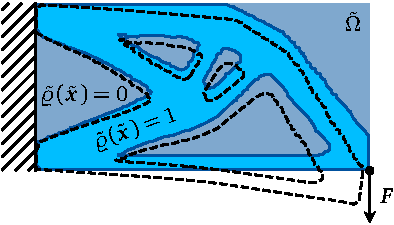
\includegraphics{topoOptExample_1}%
  \caption[%
    Example scenario for topology optimization%
  ]{%
    Example scenario for topology optimization.
    An object \emph{\textcolor{hellblau}{(light blue)}}
    is fixed on the left side
    of the object domain $\objdomain$
    \emph{\textcolor{mittelblau!50}{(darker blue)}}
    and deformed by a force $\force$, resulting in a displaced object
    \emph{(dashed).}
    The density function $\densglobal(\tilde{\*x})$ is one inside the object
    and zero outside.%
  }%
  \label{fig:topoOptExample}%
\end{SCfigure}



\subsection{Two-Scale Approach}
\label{sec:612twoScale}

\paragraph{Discretization and two-scale approach}

Of course, we cannot solve the problem \eqref{eq:topoOptProblemContinuous}
numerically,
as there are infinitely many density functions $\densglobal$.
For simplicity, we assume that $\objdomain$ is some hyper-rectangle
$\clint{\tilde{\*a}, \tilde{\*b}}
= \clint{\tilde{a}_1, \tilde{b}_1} \times \dotsb \times
\clint{\tilde{a}_{\dimobjdomain}, \tilde{b}_{\dimobjdomain}}$;
if it is not, we replace $\objdomain$ with its bounding box.
The object domain $\objdomain$ can then be split into
$M_1 \times \dotsb \times M_{\dimobjdomain}$
equally-sized and axis-aligned sub-hyper-rectangles,
which we call \term{macro-cells}
(where $M_1, \dotsc, M_{\dimobjdomain} \in \nat$).

In the \term{two-scale approach,}
we assume the material of the macro-cells to be
repetitions of infinitesimally small periodic structures
(i.e., identical for each macro-cell),
called \term{micro-cells.}
These micro-cells have a specific shape, which is parameterized by
$d$ \term{micro-cell parameters} $x_1, \dotsc, x_d$,
normalized to values in the unit interval $\clint{0, 1}$.
For instance, in two dimensions,
this shape may be an axis-aligned cross
with thicknesses $x_1$ and $x_2$, as shown in \cref{fig:twoScale}.
The choice of a suitable \term{micro-cell model}
(parametrization of the micro-cells)
depends on the optimization scenario and has to be done a priori.

\begin{figure}
  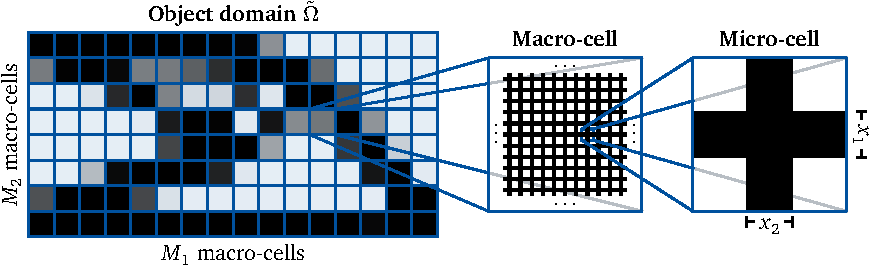
\includegraphics{twoScale_1}%
  \caption[%
    Two-scale approach for topology optimization%
  ]{%
    Two-scale approach to discretize the homogenized topology
    optimization problem in two dimensions ($\dimobjdomain = 2$).
    \emph{Left:} The object domain $\objdomain$ is
    subdivided into $M_1 \times M_2$ macro-cells,
    each with its own density \emph{(gray squares).}
    \emph{Center:} Every macro-cell is the repetition of infinitesimally small
    periodic micro-cells.
    \emph{Right:} The shape of the structure in every micro-cell is
    described by a micro-cell model with $d$ parameters $x_1, \dotsc, x_d$.
    Here, the micro-cell model is a cross with two parameters
    that represent the thickness of each crossbar.%
  }%
  \label{fig:twoScale}%
\end{figure}

\paragraph{Elasticity tensors}

Note that while the shape of all micro-cells in one macro-cell is identical,
the micro-cell parameters corresponding to different macro-cells differ
in general.
This enables varying densities in different regions of $\objdomain$.
We denote the micro-cell parameters corresponding to the $q$-th macro-cell
with $\mcp{q} = (\mcpentry{1}{q}, \dotsc, \mcpentry{d}{q}) \in
\clint{\*0, \*1} = \clint{0, 1}^d$,
where $q = 1, \dotsc, M$ and
$M \ceq M_1 \dotsm M_{\dimobjdomain}$ is the number of macro-cells.
With linear elasticity,
one can compute so-called \term{elasticity tensors} $\etensor^{(q)}$,
which encode information about the material properties
of the different macro-cells.
The elasticity tensors can be written as symmetric matrices
in $\real^{3 \times 3}$ (for $\dimobjdomain = 2$) or
in $\real^{6 \times 6}$ (for $\dimobjdomain = 3$).%
\footnote{%
  In general, the elasticity tensor is a fourth-order tensor in
  $\real^{\dimobjdomain \times \dimobjdomain \times \dimobjdomain \times \dimobjdomain}$.
  One can reduce the size of the tensor by exploiting various symmetries
  \cite{Huebner14Mehrdimensionale}
  to obtain $6$ or $21$ stiffness coefficients
  in two or three dimensions, respectively.
  These coefficients can then be expressed as a symmetric matrix.%
}
To simplify the following considerations,
we assume that $\dimobjdomain = 3$, i.e.,
$\etensor^{(q)} \in \real^{6 \times 6}$.
The elasticity tensors are usually computed as the solution of a \fem problem
\term{(micro-problem).}
Once all $\etensor^{(q)}$ are known,
we can compute the compliance value
by solving another \fem problem \term{(macro-problem),}
see \cite{Allaire04Topology} and \cite{Huebner14Mehrdimensionale}.

\vspace{-0.5em}

\paragraph{Discretized optimization problem}

The new optimization problem emerging from the
two-scale discretization process has the form
\begin{subequations}
  \label{eq:topoOptProblemDiscrete}
  \setlength{\belowdisplayskip}{5pt}%
  \begin{gather}
    \min J(\mcp{1}, \dotsc, \mcp{M}),\quad
    \mcp{1}, \dotsc, \mcp{M} \in \clint{\*0, \*1}
    \quad\text{s.t.}\quad
    \densmean(\mcp{1}, \dotsc, \mcp{M}) \le \densub,\\
    \densmean(\mcp{1}, \dotsc, \mcp{M})
    \ceq \frac{1}{M} \sum_{q=1}^M \denscell^{(q)}(\mcp{q}).
  \end{gather}
\end{subequations}
Here, $\denscell^{(q)}(\mcp{q}) \in \clint{0, 1}$ is the
density of the $q$-th macro-cell with micro-cell parameter $\mcp{q}$
(i.e., the fraction of material volume of one micro-cell
with respect to its total volume)
and $\densmean(\mcp{1}, \dotsc, \mcp{M}) \in \clint{0, 1}$
is the resulting total mean density.
This discretized optimization problem can now be implemented and
solved numerically.
